\section{Direkte Fernlokalisierung mit Bluetooth Low Energy}
\label{ch:phase3}
Für die direkte Fernlokalisierung mit Bluetooth werden dedizierte Basisstationen eingesetzt. 
Die Kommunikation zwischen Basisstation und Ortungsdienst kann durch ein LAN- oder WLAN-Netzwerk gewährleistet werden.
Die Basisstationen bestimmen des \emph{Received Signal Strength Indicator} (RSSI) eingehender Übertragungen der mobilen Enheiten und übermitteln die gemessenen Werte dann an den Ortungsdienst.
Der Ortungsdienst kann mit den gesammelten Werten die Position der mobilen Einheit berechnen.

\subsection{nRF52832}
Der nRF52832 ist eine \emph{System-on-Chip}-Lösung von Nordic Semiconductor.
Er vereint eine 32-bit ARM Cortex-M4F CPU, 512kB RAM und einen 2,4 GHz Transceiver, der Bluetooth 5.0 inklusive Low Energy und das proprietäre ANT Protokoll unterstützt \cite{nordic2017nrf}.\\
Für diese Arbeit wird ein Adafruit Feather \emph{nRF52} verwendet, der nRF52832 wird deshalb im Folgenden auf \emph{nRF52} abgekürzt.
Das Adafruit Feather \emph{nRF52} besitzt neben dem nRF52832 Spannungswandler für die 3,3 Volt Umwandlung und einen Schaltkreis für die Verwendung mit Lithium Akkus. 
Die verbaute CP2104 USB-to-Serial Schnittstelle erlaubt es, den Chip über USB zu programmieren.\\
Abbildung \ref{fig:nrf52layout} zeigt das Adafruit Feather nRF52.
Auch Nordic Semiconductor gibt einige typische Stromverbräuche für ihr \emph{System-on-Chip} an, diese sind in Tabelle \ref{table:nrf52consumption} aufgeführt.

\begin{figure}[h]
  \centering
	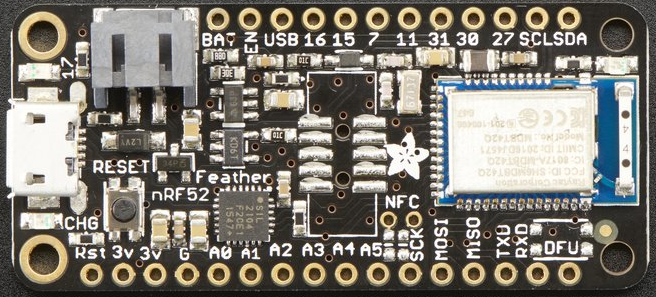
\includegraphics[width=\textwidth]{images/nrf52ada.png}
  \caption{Adafruit \emph{nRF52} Feather. Bild von Adafruit Industries\protect \footnotemark.}
  \label{fig:nrf52layout}
\end{figure}
\footnotetext{\url{https://www.adafruit.com/product/3406}}

\begin{table}[h]
  \centering
  \caption{Stromverbrauch des nRF52832 in verschiedenen Zuständen, aus \cite{nordic2017nrf}}
	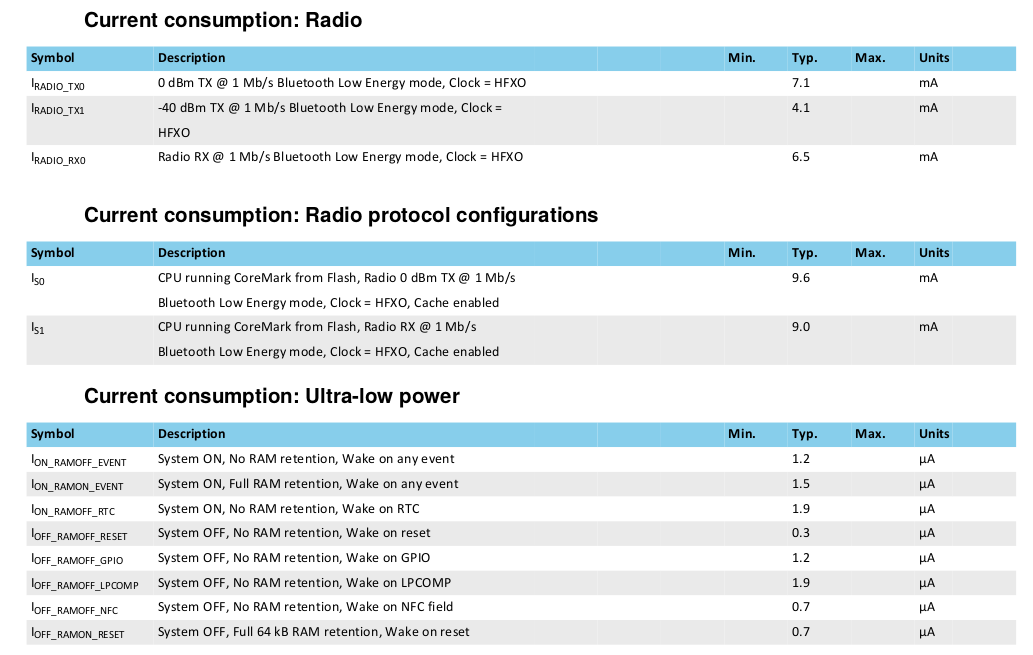
\includegraphics[width=\textwidth]{images/nrf52consumption.png}
  \label{table:nrf52consumption}
\end{table}


\subsubsection{Arduino Bluefruit nRF52 API}
Der \emph{nRF52} kann ebenfalls mit der Arduino IDE programmiert werden.\\
Adafruit stellt eine englischsprachige Anleitung zur Verwendung des \textit{Adafruit Feather nRF52 Bluefruit} mit Arduino zur Verfügung\footnote{\url{https://learn.adafruit.com/bluefruit-nrf52-feather-learning-guide?view=all}}.
Die \emph{Bluefruit nRF52} API stellt dabei Funktionen zur Verwendung von Bluetooth und Bluetooth Low Energy zur Verfügung.
Es wird die \emph{Bluefruit nRF52} API Version 0.6.0 verwendet.



\subsection{Reichweite von Bluetooth Low Energy}
Der Versuch mit BLE wurde an der selben Stelle wie der mit WLAN durchgeführt, siehe dazu Abschitt \ref{ch:phase1:sec:rangewlan}.
Es wurde allerdings ein \emph{Raspberry Pi Zero W} als Basisstation verwendet, dieser wurde auf dem \emph{LN-862} platziert, auf Abbildung \ref{fig:applacement} ist sein rotes Gehäuse zu erkennen.

\subsubsection{Methodik}
Die Reichweite wurde erneut in zwei Richtungen geprüft. 
Zum einen in Richtung der fertig gebohrten Tunnels mit wenigen Hindernissen, zum anderen in Richtung des Vortriebs durch mehrere Stahlhindernisse.
Die zwei Messtrecken werden in Abbildung \ref{fig:rangeblue} skizziert.

\begin{figure}[h!]
  \centering
	\includegraphics[width=\textwidth]{images/rangeblue.eps}
  \caption{Messtrecken zur Festellung der Reichweite von Bluetooth Low Energy.}
  \label{fig:rangeblue}
\end{figure}

Um die Abschirmung durch ein Gehäuse zu simulieren wurde eine stabile Plastikbox verwendet, leider konnte diese nicht vollends geschlossen werden.
Für die Messung wurde der Körper zwischen mobile Einheit und Basisstation gebracht und eine mobile Einheit wurde dann als "{}außer Reichweite"{} angesehen, wenn versendete Pakete der mobilen Einheit nicht mehr bei der Basisstation ankamen.
Durch das Entfernen des körperlichen Hindernisses war es möglich wieder eine Verbindung herzustellen.\\
Die bestimmten Reichweiten werden in zwei Meter Schritten angegeben, da sie mit Hilfe der zwei Meter breiten \emph{Tübbinge} bestimmt wurden.

\subsubsection{Ergebnisse}
Tabelle \ref{table:rangeblue} zeigt die Ergebnisse für den nRF52.
Das lose Auflegen des Gehäusedeckels führte zu keiner Veränderung bei der Reichweite.

\begin{table}[h]
	\centering
	\caption{Sendereichweite Bluetooth-basierter mobiler Einheiten}
	\label{table:rangeblue}
	\begin{tabular}{l|l|l|p{3cm}}
		Hardware & Aufbau & Strecke & Maximale Sendereichweite \\
		\hline
		\emph{nRF52} Feather & Offen & Wenige Hindernisse & 32 m \\
		\emph{nRF52} Feather & In Gehäuse & Wenige Hindernisse & 32 m \\
		\emph{nRF52} Feather & Offen & Viele Hindernisse & 14 m \\
		\emph{nRF52} Feather & In Gehäuse & Viele Hindernisse & 14 m \\
	\end{tabular}
\end{table}

\subsubsection{Bewertung}
Um mit 30 km/h 32 Meter zu durchqueren benötigt man 3,8 Sekunden.
Da jedoch eine hohe Erkennungszuverlässigkeit gefordert wurde, sollte das Sendeintervall niedriger gesetzt werden, es wird auf eine Sekunde gesetzt.
Damit werden auch bei einer Reichweite von nur 14 Metern auf der Tunnelbohrmaschine ausreichend viele Pakete versenden um den Verlust einzelner zu kompensieren.

\subsection{BLE-Advertising-Implementierung}
\label{ch:phase3:sec:advertising}
Die \emph{Bluetooth-Low-Energy-Implementierung} ist an die Arbeit von Jianyong et al. angelehnt.
Es wird immer nach Ablauf des Sendeintervalls ein \emph{Advertising} Paket gesendet.\\
In der Praxis wird dazu das \emph{Advertising}-Intervall entsprechend gesetzt, dabei handelt es sich um einen in Bluetooth 4.0 spezifizierten Parameter für die Häufigkeit des \emph{Advertisings}.
Da die \emph{Bluefruit} \emph{nRF52} API keine Funktion zur Änderung dieses Wertes zur Verfügung stellt muss er direkt geändert werden.
Die entsprechende \emph{BLEAdvertising}-Klasse ist in \\\texttt{/.arduino15/packages/adafruit/hardware/nrf52/0.6.0/libraries/}\\\texttt{Bluefruit52Lib/src} zu finden. \\
In \texttt{BLEAdvertising.cpp} ist \texttt{GAP\_ADV\_INTERVAL\_MS} auf 20 Millisekunden gesetzt, dieser Wert sollte erhöht werden, um den Stromverbrauch zu senken.
Beim \emph{nRF52} handelt es sich um ein Klasse 2 Bluetooth-Gerät mit einer maximalen Sendeleistung bis 4 dBm.
Das Sendeintervall wird etsprechend der Untersuchung der Reichweite und maximalen Bewegungsgeschwindigkeit von 30 km/h auf eine Sekunde gesetzt, in dieser Zeit kann sich ein Mitarbeiter maximal 9 Meter bewegen.\\
Es sollte erneut eine Voruntersuchung des Verbrauchs mit dem Muker \emph{TM103} USB-Power-Meter vorgenommen werden.
Diser ist aber nicht in der Lage den Stromverbrauch des \emph{nRF52} zu messen.
Die Sendeabschnitte sind zu kurz um einen messbaren Stromverbrauch zu erzeugen.\\
Deshalb wird zunächst Abbildung \ref{table:nrf52consumption} für eine theoretische Betrachtung des Verbrauchs herangezogen werden. 




\subsection{Untersuchung des Stromverbrauchs}
Der Stromverbrauch soll mit dem INA219 genauer bestimmt werden, der INA219 und die verwendete Methodik werden in Abschnitt \ref{ch:phase1:sec:energie} beschrieben.

\subsubsection{Theoretische Stromverbrauchsabschätzung}
Für die Zeit in der nicht gesendet wird, wird der Zustand $I_{ON\_RAMOFF\_RTC}$ angenommen, da dieser den höchsten Verbrauch aufweist.
Für die Sendezeit wird $I_{RADIO\_TX0}$ angenommen, für ein \emph{Advertising}-Paket, welches zusätzlich den Gerätenamen "{}TestTag"{} versendet, werden 24 Bytes (192 Bit) gesendet.
Um die Kollisionsvermeidung einzufügen werden vorher 2000 Bit im Zustand $I_{RADIO\_RX0}$ empfangen, der die restliche Zeit wird in $I_{ON\_RAMOFF\_RTC}$ verbracht. 
Es müssen ebenfalls die weiteren Komponenten auf dem Feather bedacht werden. 
Adafruit gibt für den Spannungswandler einen Verbrauch von 55 Mikroamper und für den Lithium-Polymer-Ladeschaltkreis einen Verbrauch von bis zu 100 Mikroamper an \cite{fried2016lora}. 
Der Verbrauch des anderen Komponenten des Feather wird daher konservativ auf 155 Mikroamper geschätzt.\\[1cm]

$y = (1s-\frac{Bits\_gesendet}{1000000 b/s} - \frac{Bits\_empfangen}{1000000 b/s}) * (I_{ON\_RAMOFF\_RTC} + 155 {\mu}A) + \frac{Bits\_gesendet}{1000000 b/s} * I_{RADIO\_RX0} + \frac{Bits\_empfangen}{1000000 b/s} * I_{RADIO\_RX0}$\\[0.5cm]
$y = (1s - 0,000192s - 0,002s) * 0,1569mA + 0,000192 * 7,1mA + 0,002 * 6,5mA$\\[0.5cm]
$y \approx 0,156556mA + 0,001363mA + 0,013mA = 0,170919mA$ \\[1cm]

\subsubsection{Tatsächlicher Stromverbrauch von BLE}
\label{ch:phase3:sec:powerble}
Abbildung \ref{fig:blue} zeigt den Lastverlauf für den Start einer mobilen Einheit mit Bluetooth-Low-Energy-Advertising.\\
Zu Beginn ist eine Startphase zu erkennen, ab 2 Sekunden nach Start des Experiments ist dann das regelmäßige Muster aus Verbrauch im Ruhezustand und kurzen Verbrauchsspitzen beim Senden zu erkennen.
Die Kürze des Sendevorgangs bedingt die starke Schwankung bei den Lastspitzen, die Samplingrate von 333 Hz reicht hier offenbar nicht aus um dem Sendevorgang vollständig zu erfassen.\\

\begin{figure}[h!]
  \centering
	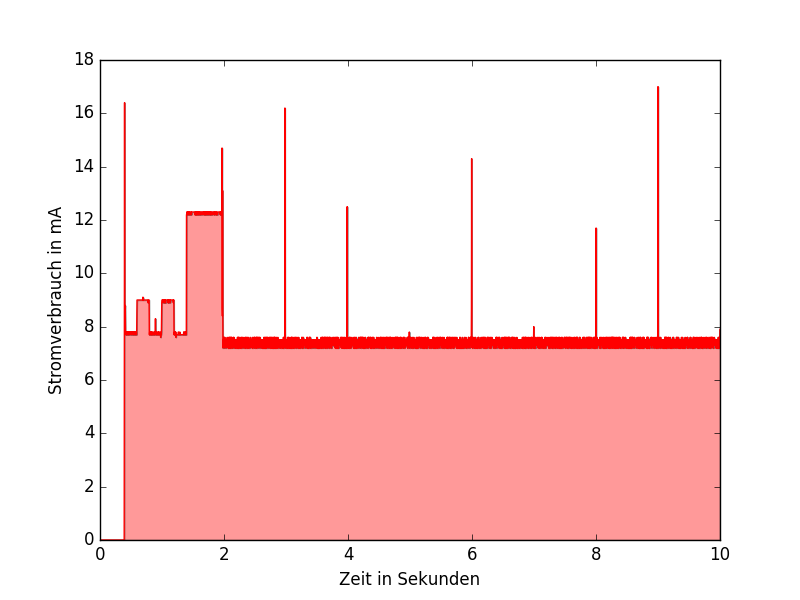
\includegraphics[width=\textwidth]{plots/blue.png}
  \caption{Stromverbrauchskurve einer Implementierung von Bluetooth-Low-Energy-Advertising.}
  \label{fig:blue}
\end{figure}

Hauptverbrauch liegt jedoch in den 7,2 bis 7,6 Milliamper im Ruhezustand, leider ist in diesem Fall kein einzelnes Modul vorhanden, es kann nur auf dem \emph{nRF52} Feather gemessen werden.
Tabelle \ref{table:blueina} zeigt deshalb neben dem gemessenen Verbrauch den normalisierten Stromverbrauch, dafür wurde der Verbrauch im Ruhezustand subtrahiert. 
Dies beschränkt den Verbrauch auf den für die tatsächliche Funktion nötigen Anteil.

\begin{table}[h!]
	\centering
	\caption{Stromverbrauch mobiler Einheiten mit Bluetooth-Low-Energy-Advertising}
	\label{table:blueina}
	\begin{tabular}{p{3.5cm}|p{5cm}|p{2.5cm}|p{2.5cm}}
		Hardware & Programm & $\varnothing$ Verbrauch in mA (normalisiert) & Laufzeit in Stunden\\
		\hline
		\emph{nRF52} Feather & Bluetooth-Low-Energy-Advertising & 7,37 (0,04) & 190\\
	\end{tabular}
\end{table}

